\section{Experimental Results}
\label{sec:moe_results}
We demonstrate the efficacy of the mixture of expert controllers in simulation
and real-world experiments.
%
In the first case study, we learn a gating network that switches between two
unstable closed-loop systems to result in a piecewise-stable system.
%
Then, we find switching MOE controllers to swing up the classical cartpole
mechanism enclosed with wall barriers.
%

\subsection{Stable Switching Between Unstable Systems}

Suppose we have two linear closed-loop systems of the form 
\begin{equation}
    \begin{gathered}
        \dot{x} = A_1x = \bmat{0 & -1 \\ 2 & 0}x \\
        \dot{x} = A_2x = \bmat{0 & -2 \\ 1 & 0}x.
    \end{gathered}
    \label{eq:unstable_closedloop}
\end{equation}
%
Even if both systems are unstable, it is possible to find a state-dependent
switching rule that makes the resulting switched system
stable~\cite{liberzon2003switching}. 
%
We aim to learn the parameters $\psi$ of the gating network $P(x;
\psi)$ such that the switching system converges to the desired equilibrium $x^*
= (0, 0)$.
%
The gating network is a fully-connected neural net with one hidden layer (2 input states 
\rightarrow 6 neurons \rightarrow 4 outputs) and an \textsc{Elu} activation
function~\cite{clevert2015fast}.
%
We constrain the maximum number of state partitions to $4$.
%
Each state partition has a corresponding controller parameter $\theta_i \in
\mathbb{R}$. 
%
The control law is a sample from the Bernoulli probability distribution
\begin{align}
    u(\theta_i) = \begin{cases}
       0, & \theta_i > \frac{1}{2}, \\
       1, & \theta_i \leq \frac{1}{2},
    \end{cases}
\end{align}
\noindent where $u = 0$ corresponds to the first dynamics $\dot{x} = A_1
x$ and $u=1$ corresponds to $\dot{x} = A_2x$.
%
We use the \textsc{Sigmoid} activation function to limit $\theta_i$ between 0
and 1.
%
We generate a trajectory following the procedure in
Algorithm~\eqref{algo:switching_A1A2}.
%
The likelihood is modified to account for the probabilistic control as
\begin{align*}
    \mathbb{L}(\phi) = \int_{0}^{T} \Biggl( \sum_{i=1}^{N_F} - \theta_i \ell \Bigl(x(t), u(\theta_i) \Bigr) - (1- \theta_i)\ell \Bigl(x(t), u(1-\theta_i) \Bigr) +
    \ln  P\Bigl(c_i = i | x(t), \psi \Bigr)  \Biggr) \dd t.
\end{align*}

\begin{algorithm}
    \setstretch{1.2}
      \caption{Stable Switching between Unstable Systems}
      \label{algo:switching_A1A2}
      \small
      \hspace*{\algorithmicindent} \textbf{Input}: $x(0)$
      \begin{algorithmic}[1]
        \State $\phi \leftarrow  [x(0)]$ \Comment{Initial States}
          % \algrenewcommand\algorithmicindent{0em} % No indent
            \For{$t \in 0:\Delta t:T$} 
              \State $i \sim \text{Categorical}\Bigl(P(x(t); \psi)\Bigr)$ \Comment{Sample a bin number}
              \State $u \sim \text{Bernoulli} \Bigl(\textrm{Sigmoid}(\theta_i) \Bigr)$      
              \State $x(t+\Delta t) = (1-u)A_1x(t) + u \; A_2x(t) $
              \State $\phi \leftarrow \phi \cup [x(t+\Delta t)]$
            \EndFor
          \State \textbf{return} $\phi$
      \end{algorithmic}
  \end{algorithm}
  
%
The resulting switching system is shown in Figure~\ref{fig:final_switching}.
%
The training uses only 3 out of the 4 state partitions available.
%
The state partition in Figure~\ref{fig:final_switching} matches the analytical
solution to the stable switching system given as~\cite{liberzon2003switching}
\begin{equation*}
    \dot{x} = \begin{cases}
        A_1x, \; x_1x_2 \leq 0, \\
        A_2x, \; x_1x_2 > 0.
    \end{cases}
\end{equation*}
\noindent where $x=[x_1, x_2]$.
%
The training progress is shown in Figure~\ref{fig:switching_training}.
%
The three rows in the figure depict the performance of the training after 0, 200
and 1400 parameter updates, respectively.
%
The sampled trajectory on the top left figure shows that the initial parameters
created unstable switching between the two systems.
%
After only few parameter updates, the training finds a stable switching
mechanism, but it does not yet converge to the desired equilibrium $x^*$.
%
The explorative state sampling technique visits states close to the desired
equilibrium, allowing the training to learn the distinct boundaries of each
partition at the origin. 
\begin{figure}[H]
    \centering
    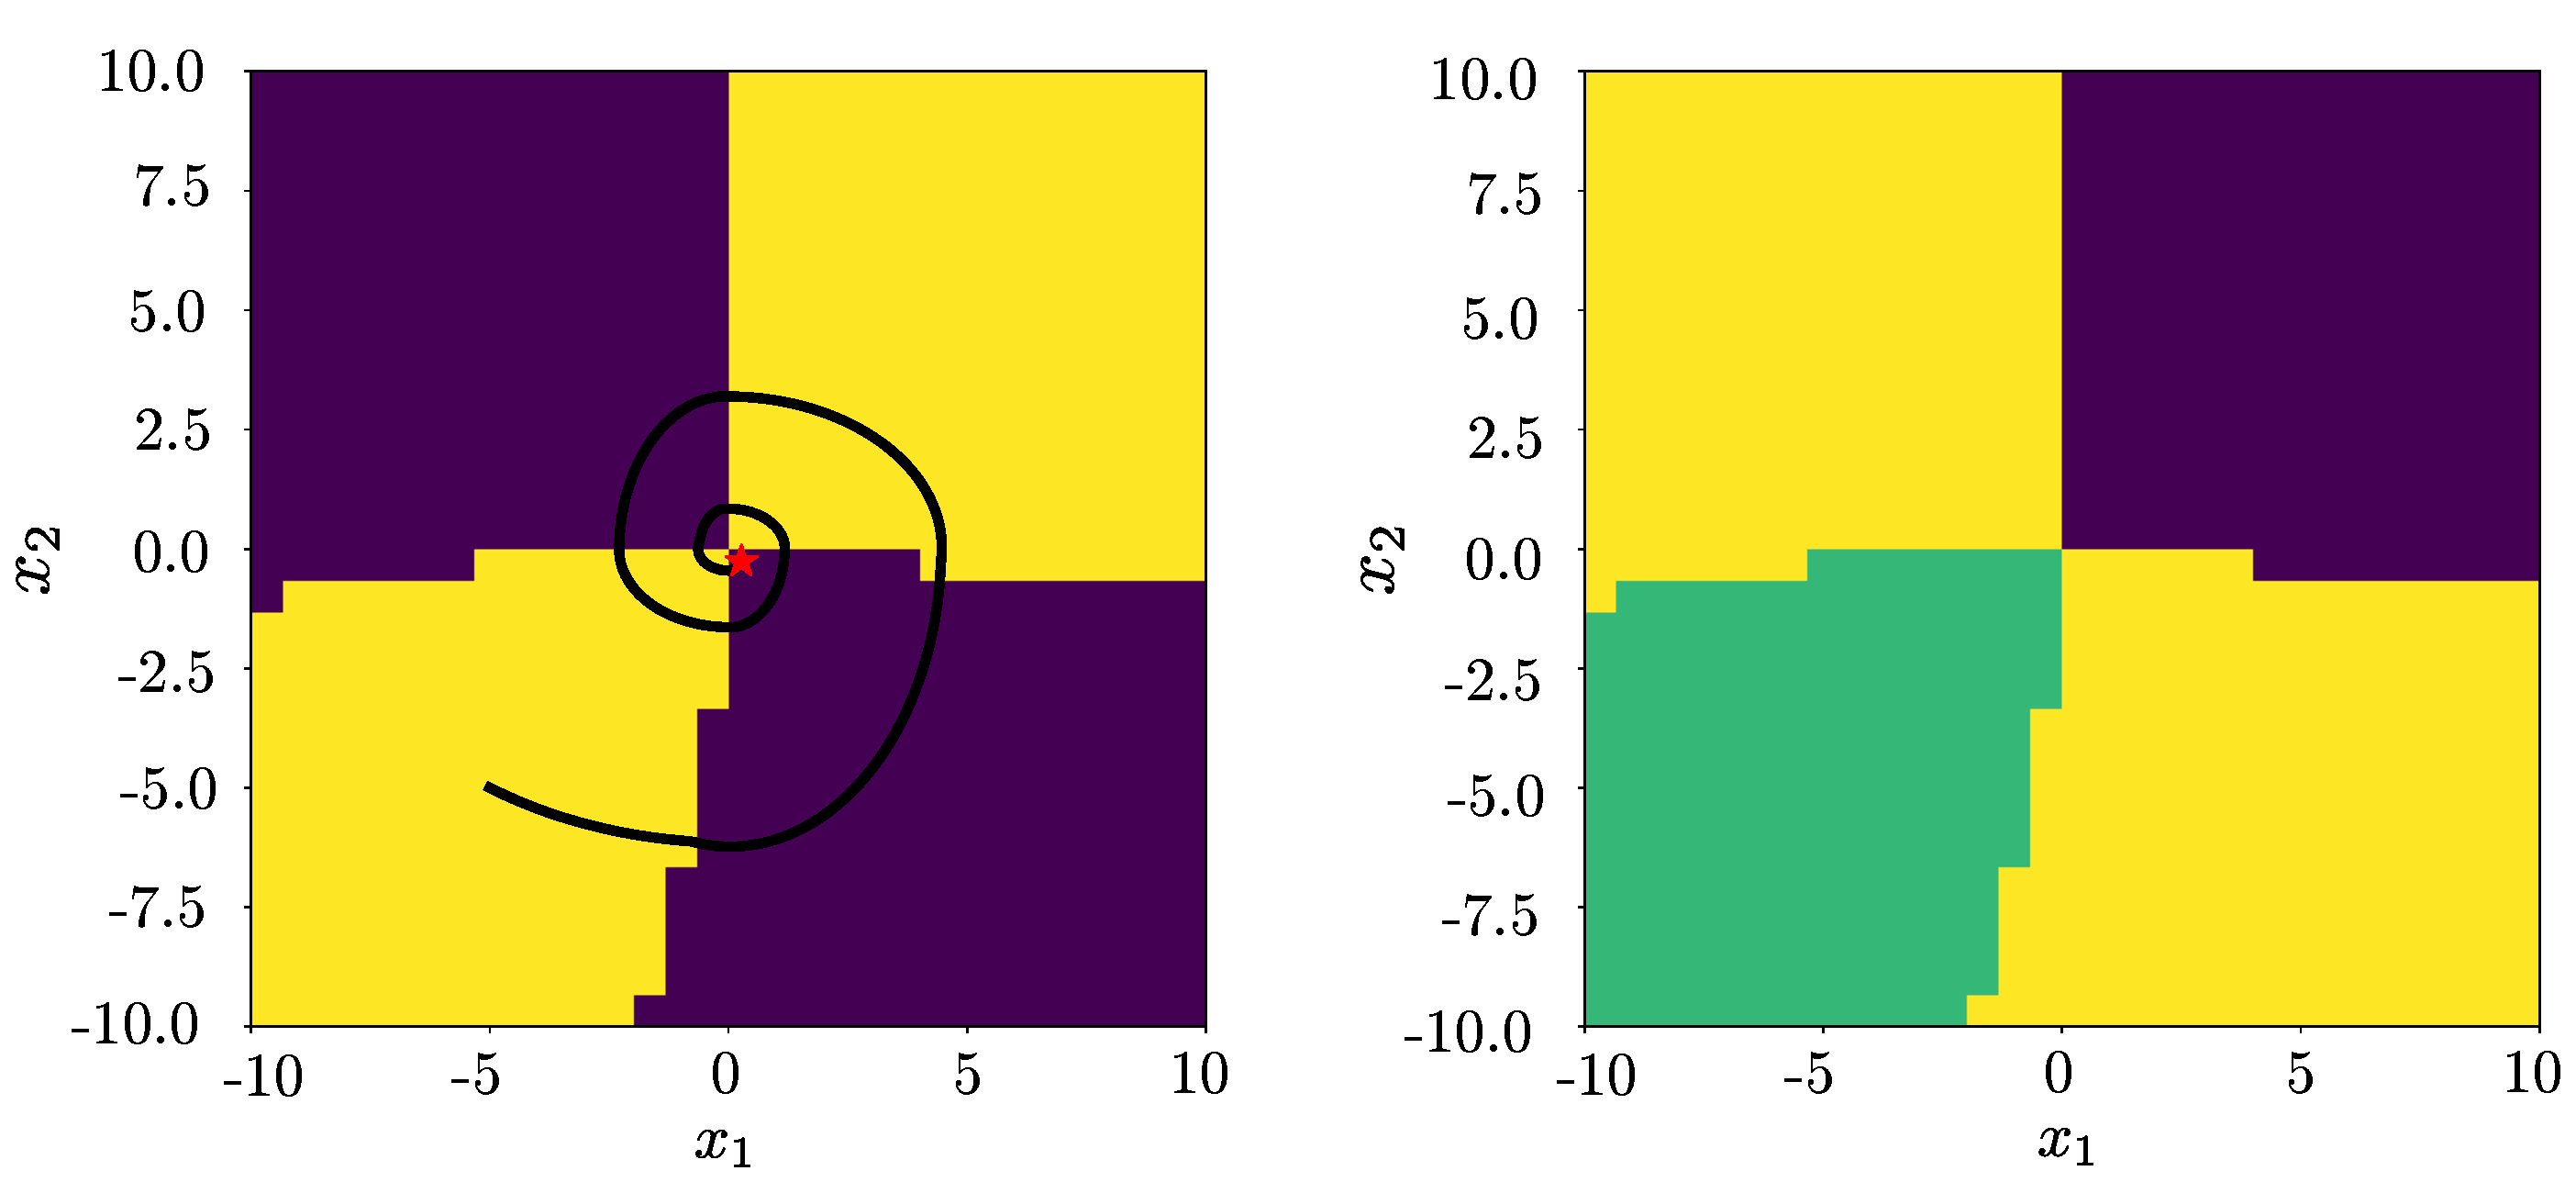
\includegraphics[width=0.92\linewidth]{switching_results.eps}
    \caption{Final stable switching system. Left: Control input $u=\{0, 1\}$ in
    the state space. Purple corresponds to $u=0$ or $\dot{x} = A_1x$. Yellow
    corresponds to $u=1$ or $\dot{x} = A_2x$. The trajectory starts at $x_0=[-5,
    -5]$ and converges to the origin shown by the red star. Right: State
    partition from the output of the gating network. The training converged to 3
    state partitions that can stabilize the system.}
    \label{fig:final_switching}
\end{figure}

\begin{figure}[H]
    \centering
    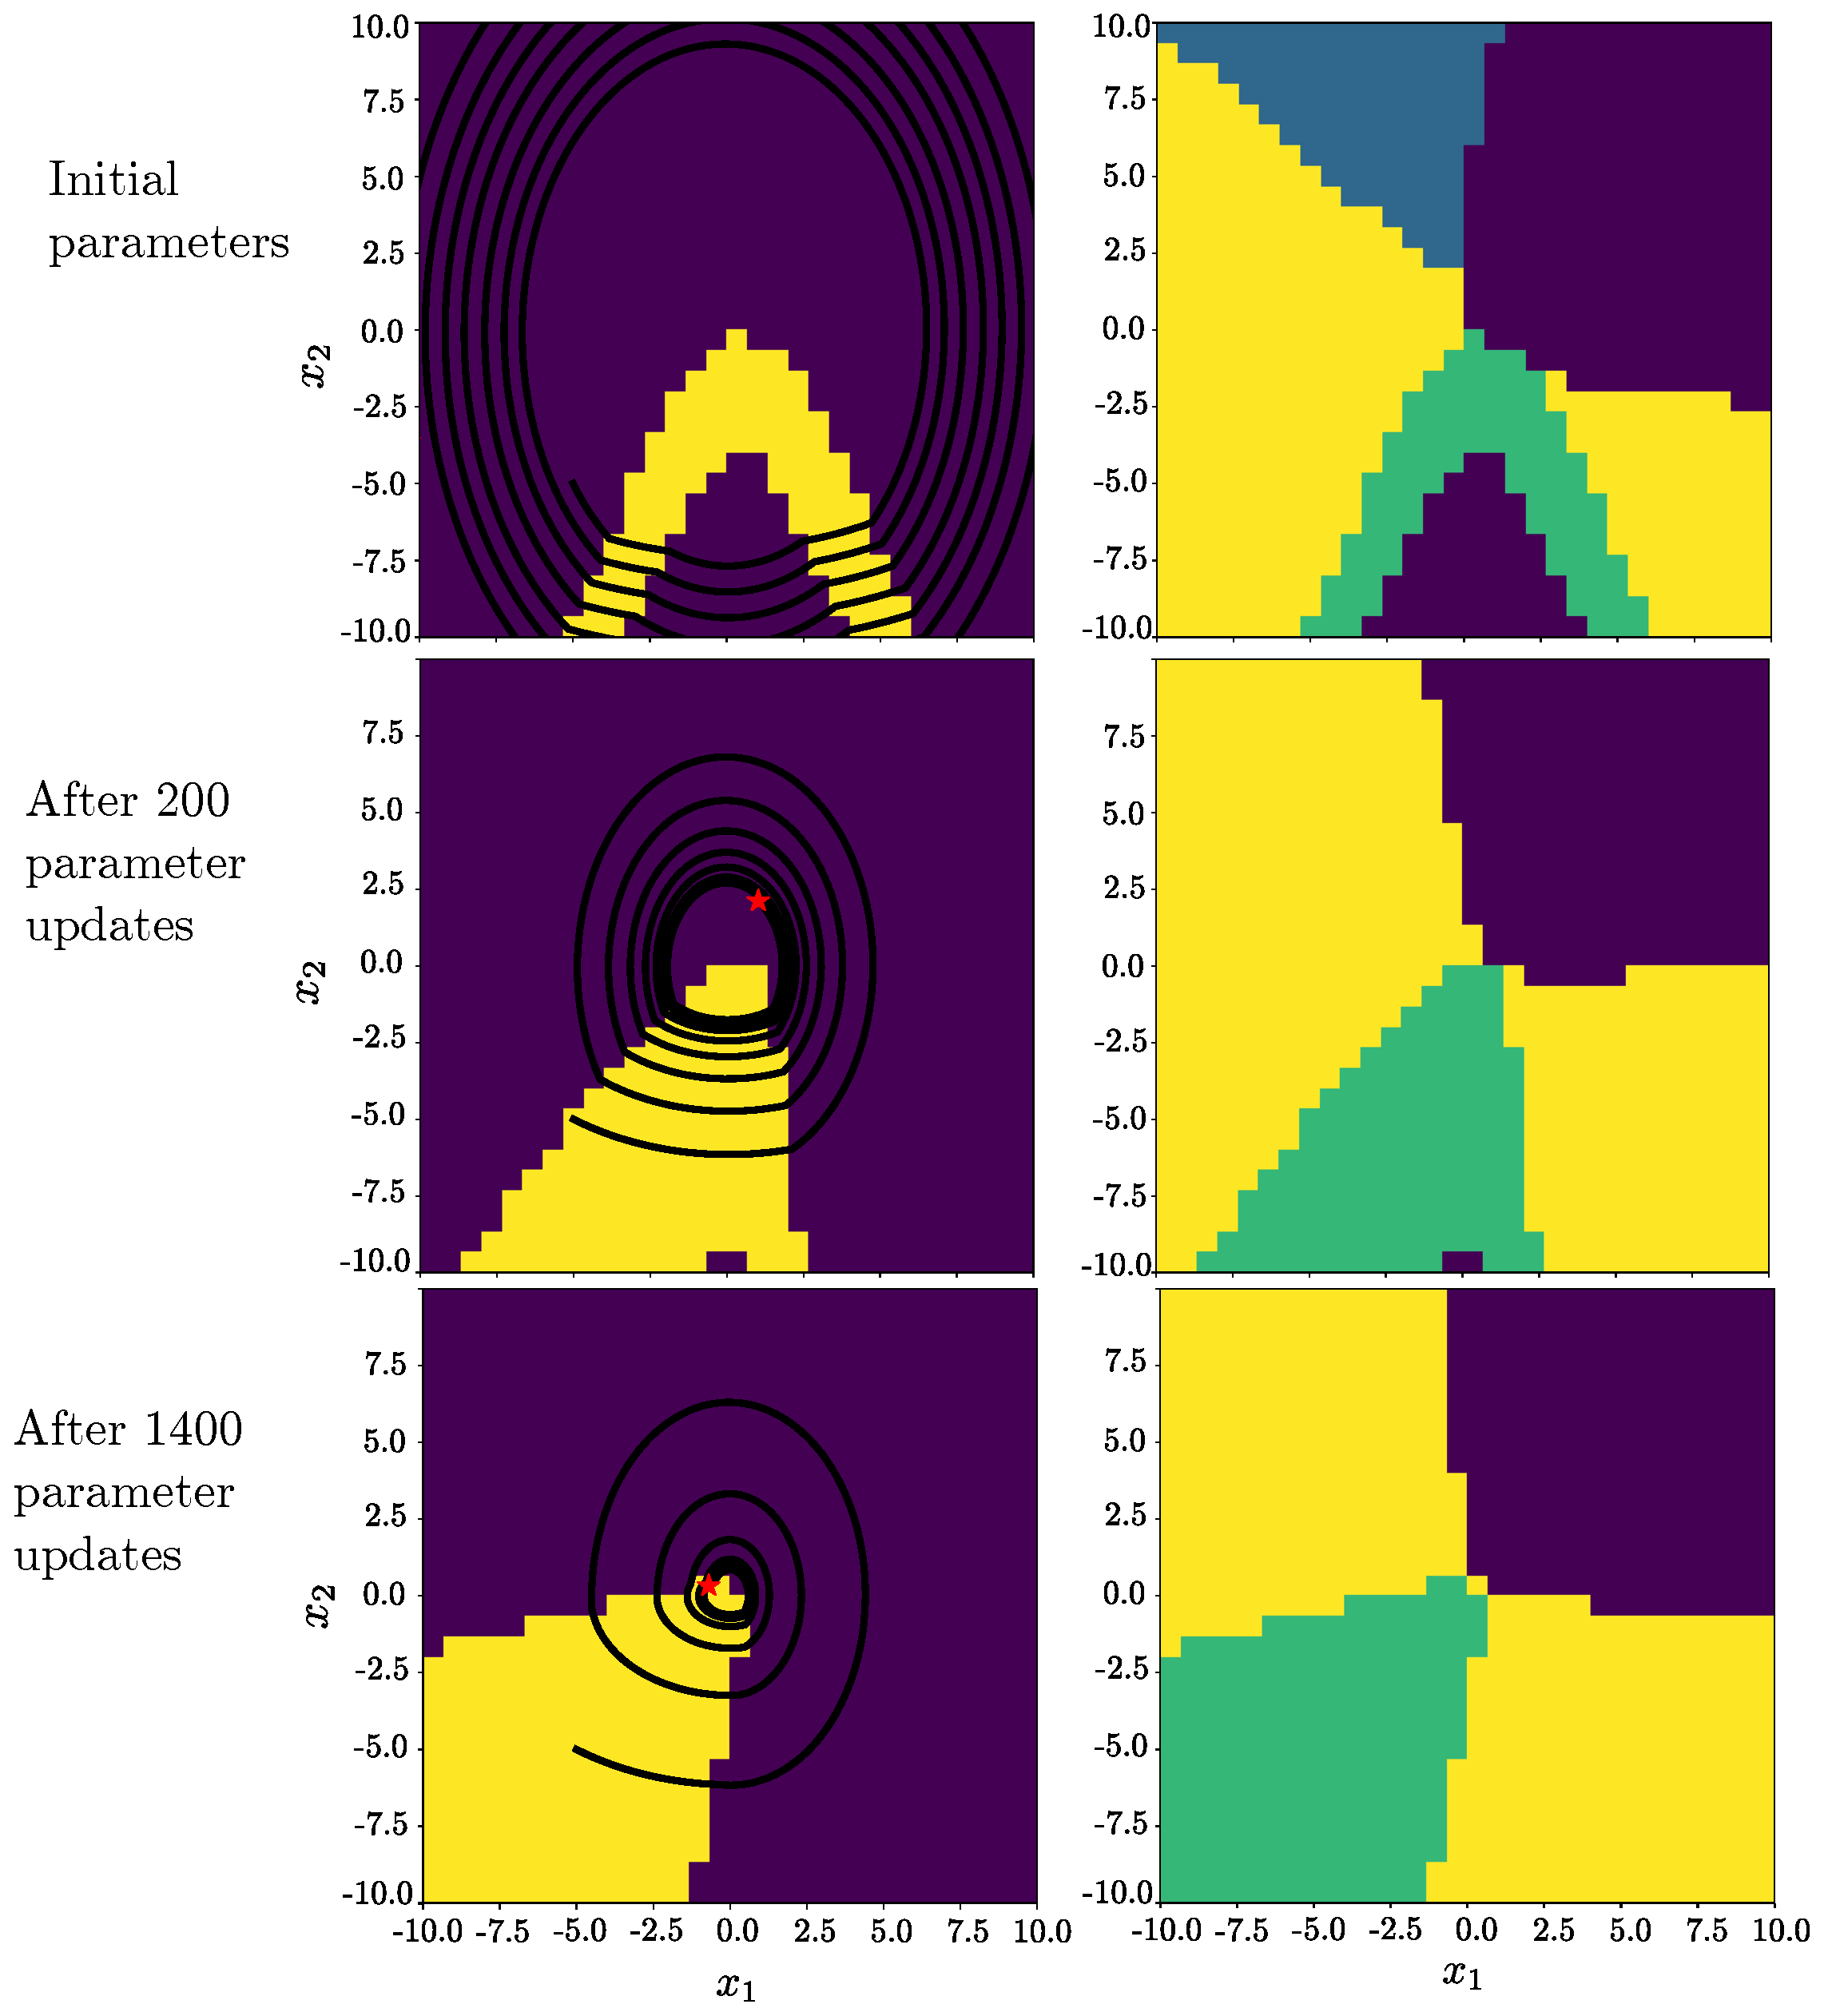
\includegraphics[width=0.87\linewidth]{switching_training.eps}
    \caption{Training progress. Top row: the control and state partition at the
    initial parameters. Second row: after 200 parameter updates. Third row:
    after 1400 parameter updates. The final solution is shown in
    Figure~\ref{fig:final_switching}}
    \label{fig:switching_training}
\end{figure} 
%%%%%%%%%%%%%%%%%%%%%%%%%%%%%%%%%%%%%%%%%%%%%%%%%%%%%%%%%%%%%%%%%%%%%%%%%%%%%%%%%%%%%%%%
\subsection{Cartpole with Wall Contacts}
\label{ssec:cartpole_with_walls}

In this section, we take the classical cartpole swing-up problem and introduce
contact events from two barriers as shown Figure~\ref{fig:cartpole_contact}. 
%
We demonstrate the performance of the mixture of expert controllers in
simulation and real-world experiments.
%
Lastly, we compare the performance of the MOE controllers against
a single swing-up controller. 


\subsubsection{System Model}
\label{sssec:cartpole_model}

The cartpole system consists of a freely rotating pendulum link hinged on an
actuated cart.
%
The setup is enclosed by two rigid walls hanging $0.2$m from the bottom of the
cart.
%
The objective is to use the control authority on the cart in order to swing-up
the passive pendulum to the upright.
%
The pendulum spans length of $l=0.2$m and its mass $m_c = 0.75$kg is
concentrated at the distance $l_{cm}=\nicefrac{l}{2}$ from the hinge.
%
The cart alone has a mass of $m_p=0.165$ kg. The viscous friction in the cart
wheels is characterized by the coefficient $b=1.2$ \nicefrac{N $\cdot$ sec}{m}.
%
The dynamics of the system
is given by~\eqref{eq:hybrid_dynamics} where 
\begin{equation}
    \begin{gathered}
        M(q) = \bmat{m_c + m_p & -m_p+l_{cm} \cos(\theta_p) \\
        -m_pl_{cm}\cos(\theta_p) & m_p l_{cm}^2+I_1} \\
        C(q, \dot{q}) = \bmat{b  & m_pl_{cm}\sin(\theta_p) \\
                -m_p\sin(\theta_p)/2 & 0} \\
        G(q) = \bmat{0 & -m_pg l_{cm} \sin(\theta_p)}^\top \\
        B = [1 \; 0]^\top
    \end{gathered}
\end{equation}
\noindent where $q = [x_c; \theta_p]$, $x_c$ is the location of the cart, $\theta_p$
is the angle of the pendulum from the vertical and $g$ is the acceleration due
to gravity. 
%
There are a total of $k=10$ contact events between the pendulum and the sides of
the walls.
%
We integrate closed-loop trajectories with Moreau time stepping algorithm
outlined in Algorithm~\eqref{algo:moreau} with an integration time step $\Delta
t=0.001$.
%

\subsubsection{Training}
\label{sssec:cartpole_training}

The goal is to learn mixture of expert controllers that stabilize the system at
$x^* = (q^*, \dot{q})^* = (0, 0)$.
%
Once the system reaches within a small neighborhood of $x^*$, we employ Linear
Quadratic Regulator (LQR) to stabilize at the desired equilibrium.
%
We use minimum trajectory loss (MTL) discussed in
Section~\ref{sssec:performance_objective} with time horizon $T=1.5$s.
%
In each parameter update, we sample $N_{\mathcal{D}}=4$ initial states through
greedy and explorative techniques.
%
The gating network is a fully-connected neural net with two hidden layers (state input
\rightarrow 4 neurons \rightarrow 3 neurons \rightarrow  1 output).
% 
We constrain the maximum number of state partitions to 3.
%
There are a total of 3 neural net experts, each corresponding to a state
partition.
%
The experts are fully-connected neural net with two hidden layers (state input
\rightarrow 10 neurons \rightarrow 4 neurons \rightarrow  1 output).
%
The output of the experts correspond to the force applied on the cart.


\begin{figure}[H]
    \centering
    \includegraphics[width=0.6\linewidth]{MOEfirstImpact.png}
    \caption{Cartpole with wall contacts}
    \label{fig:cartpole_contact}
\end{figure}

\subsubsection{Results}

We demonstrate the performance of the MOE controllers in simulation and hardware. 
%
The hardware is set up as shown in the Figure~\ref{fig:cartpole_hardware}.
% 
The cart uses a rack and pinion mechanism to translate on the track with zero-slip.
%
One of the wheels of the cart is attached to an optical encoder, from which we
can estimate the position and velocity of the cart.
%
There is also an optical encoder rigidly attached to the pendulum link,
reporting its orientation. 
%
% Both encoders with resolution $4096$
% \nicefrac{pulses}{revolution}.
%
We use MATLAB/Simulink to evaluate the neural nets and pass voltage commands to
the DC-motor.
%
We convert the force commands output by the MOE controllers into voltage
commands $V(t)$ as follows.
\begin{align*}
    V(t) = \frac{u(x(t); \psi, \theta) + A_m \dot{x}_c}{B_m}
\end{align*} 
\noindent where $A_m$ and $B_m$ consist of system parameters of the motor.

Figure~\ref{fig:cartpole_trajectory} shows a trajectory generated by the MOE
controllers in simulation and hardware.
%
The blue contours represent the level sets of the control input at the
pre-impact and post-impact states.
%
The solid line splitting the state space horizontally in half shows the boundary
between two state partitions.
%
Even though the gating network can provide up to three state partitions, the
training converges to utilizing only two.
%
Figure~\ref{fig:cartpole_trajectory} shows that the system successfully avoids
contacts during the swing-up phase, which otherwise would have prevented the
pendulum from pumping energy from the downward equilibrium.
%
By the time the pendulum approaches the upright equilibrium, it is moving at
such high speed that LQR cannot stabilize it.
%
But from several trajectories, we have observed that the system leverages the
impact from the wall to lower the speed of the pendulum.
%
Then, the control law switches between experts as the velocity jumps due to impact.
%
The magnitude of the control is such that the MOE controllers apply rapid
braking during contact, allowing LQR to catch the pendulum post-impact.
%
The MOE controllers achieve successful swing-up in simulation and real-world,
proving the accuracy in the contact modelling and the robustness of the
controllers.


\begin{figure}[H]
    \centering
    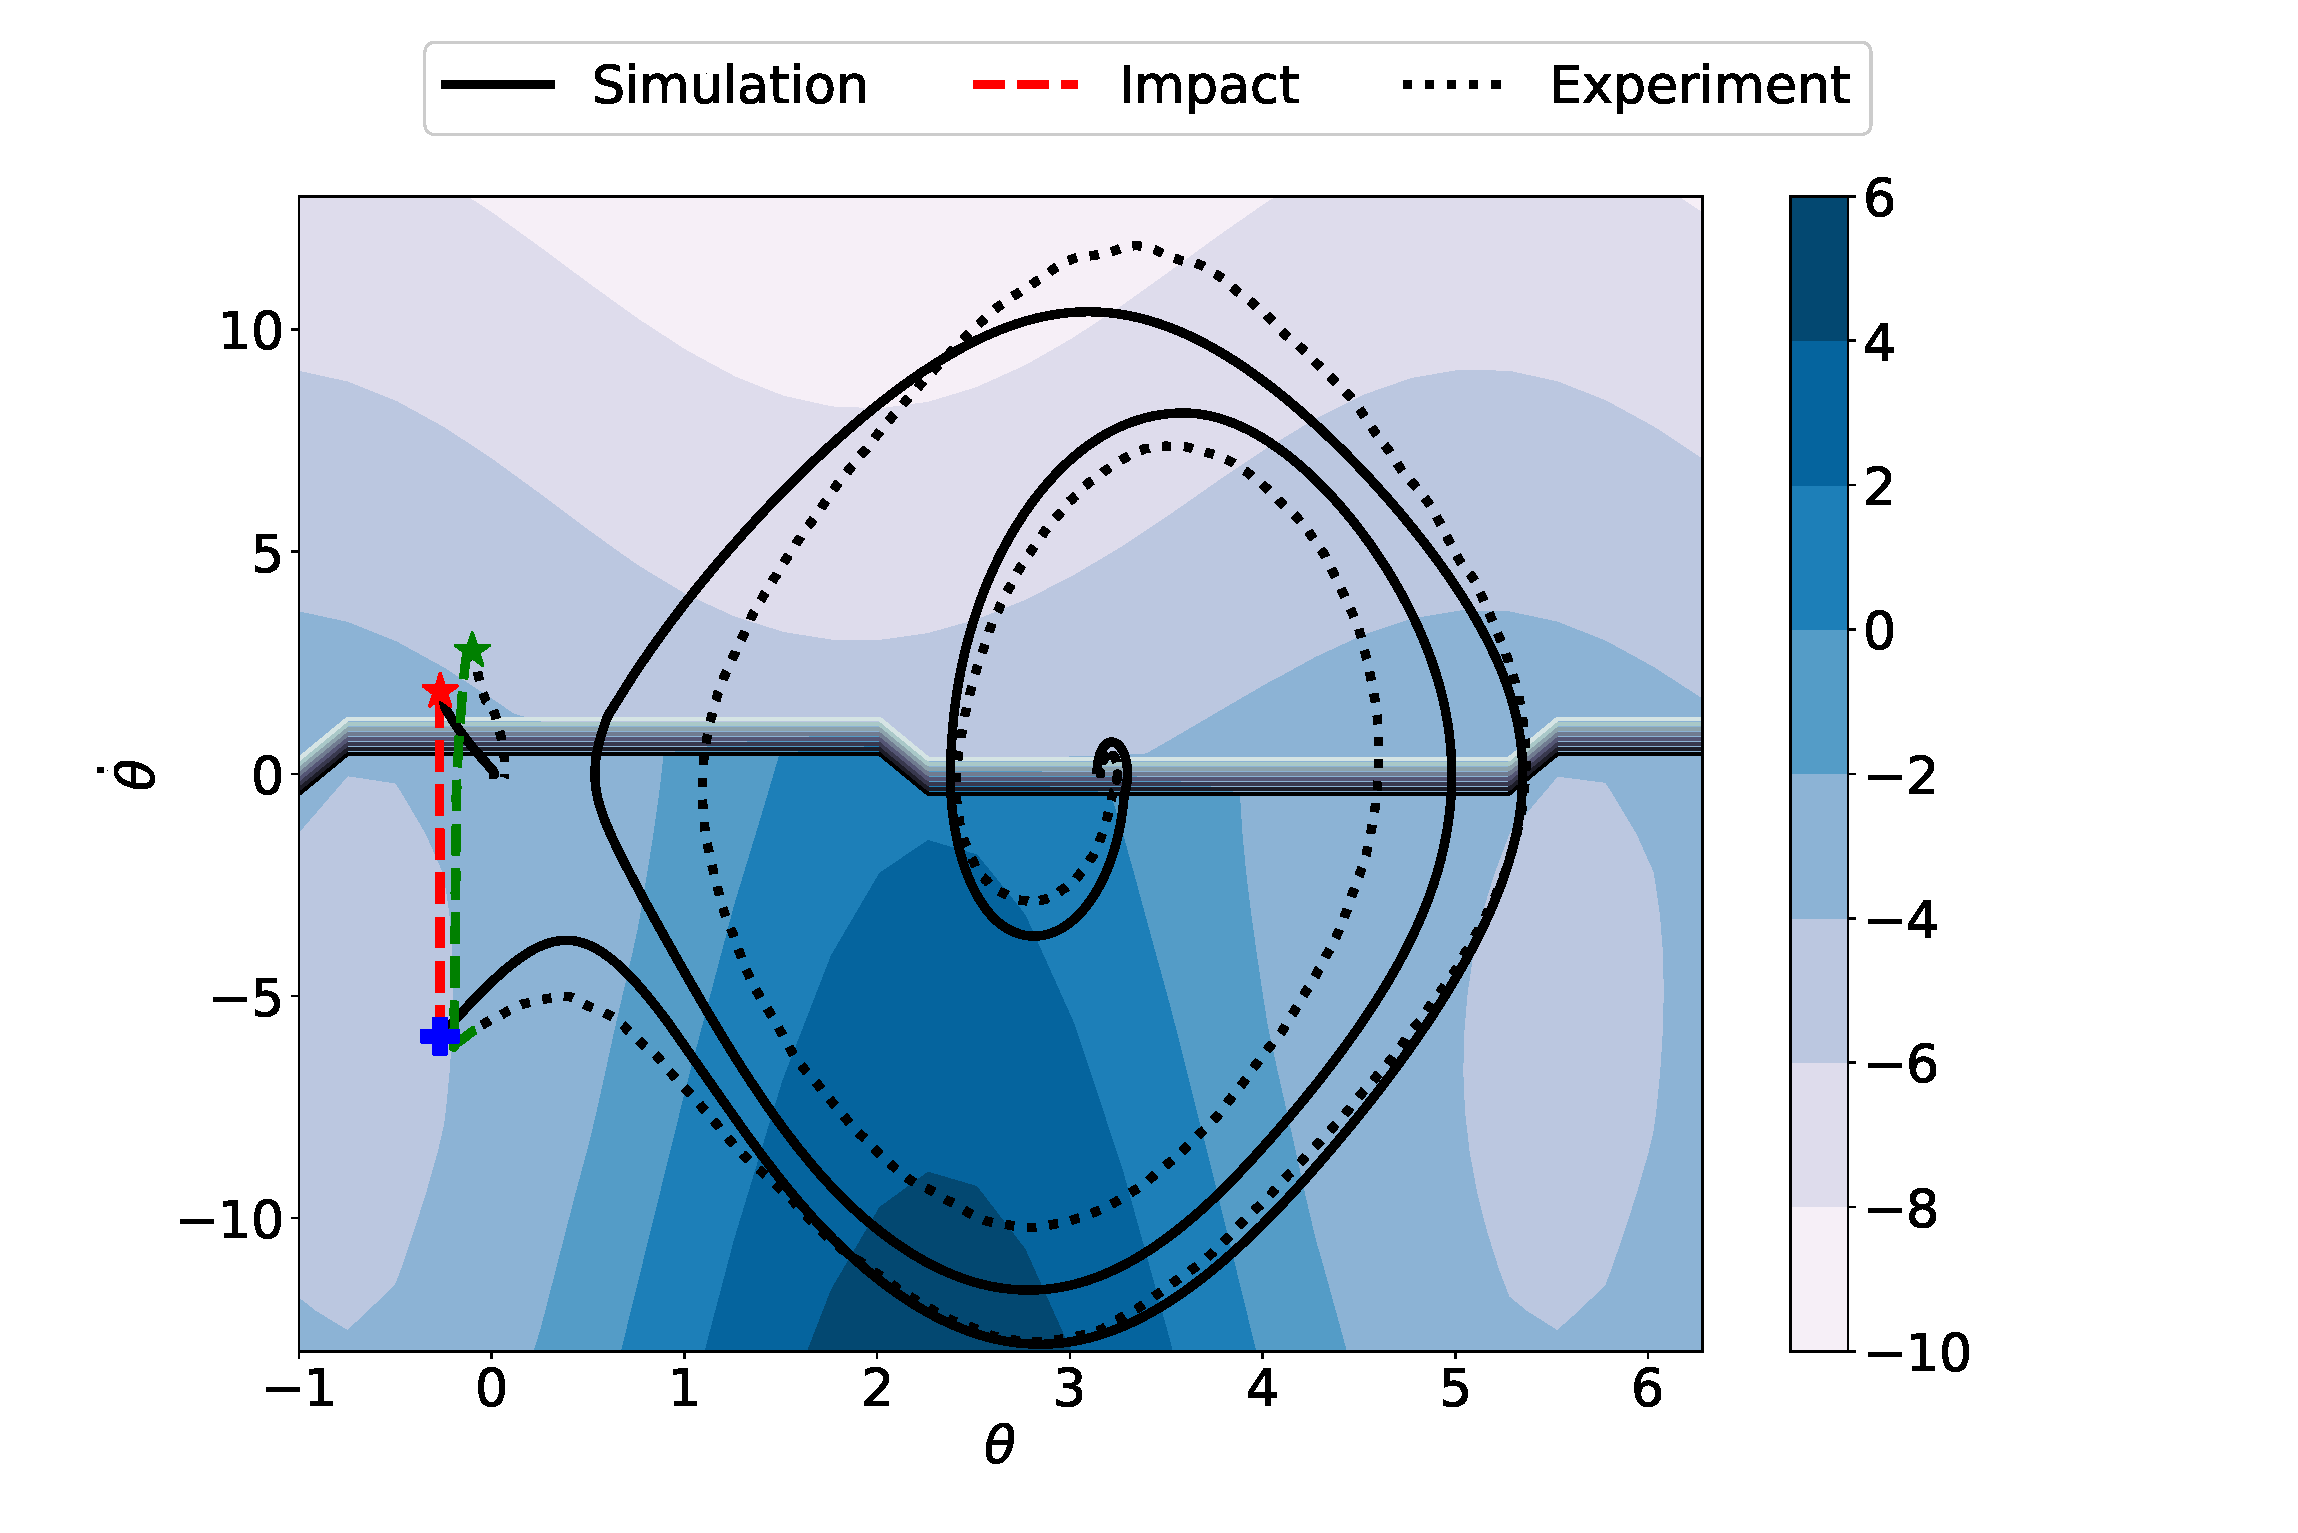
\includegraphics[width=1.0\linewidth]{moe_traj_control.eps}
    \caption{A sample trajectory starting from downward equilibrium at rest.
    The contours correspond to the outputs of the MOE controllers during impact
    ($x_c=0.36m, \dot{x}_c = 0\nicefrac{m}{s}$). The solid line
    splitting the state space horizontally in half shows the boundary between
    the two state partitions. The state partition shows that the controller must
    switch from one expert to another in order to catch the pendulum
    post-impact.}
    \label{fig:cartpole_trajectory}
\end{figure}

Figure~\ref{fig:gapContour} shows the relationship between the gap function and
the state partitions.
%
The red lines represent the boundaries of the state partitions and the contour
depicts the level sets of the gap function.
%
Notice that the states within the boundaries of the red lines have large gap
values, hence contact events do not occur in this region.
%
This shows that the gating network has dedicated one expert for states with low
risk of contact.
%
The regions outside the red boundaries correspond to the second expert, which is
activated to prevent contact during swing-up and to catch the pendulum just
after impact, as shown in the trajectory of
Figure~\ref{fig:cartpole_trajectory}.
%
This demonstrates that the state partition depends on the occurrence of contact
events.
%
Moreover, the multi-modal nature of MOE controllers allow us to leverage the
advantages or prevent the adverse effects of contacts and impacts.

\begin{figure}[H]
    \centering
    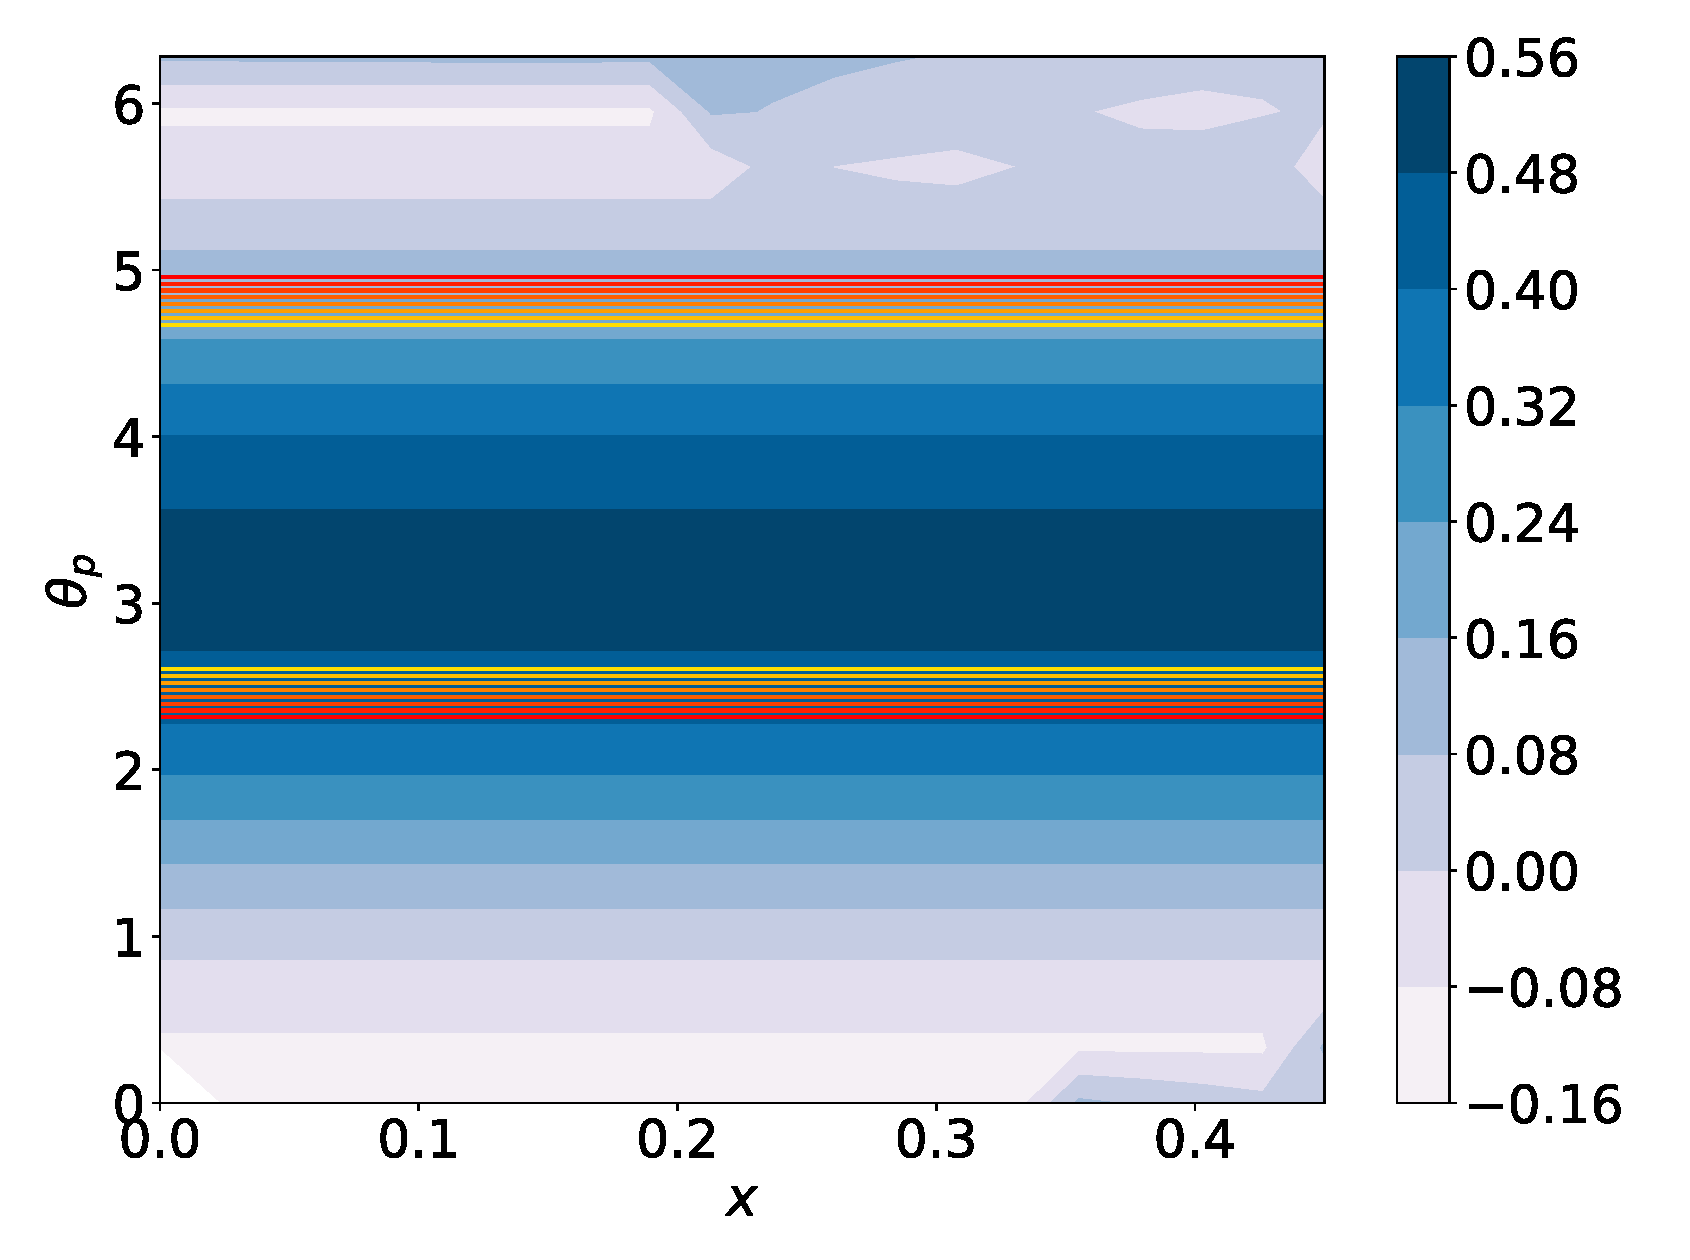
\includegraphics[width=0.7\linewidth]{gapContourAndBins.eps}
    \caption{The blue contours represent the level sets of the gap function. The red lines show the boundaries of the state partition. There are a total of two experts, one is active between the red boundaries and the other is responsible for regions outside the red lines.}
    \label{fig:gapContour}
\end{figure}


Lastly, we compare the performance of the MOE controllers against a single controller.
%
This controller is parameterized by a neural net (state input \rightarrow 10
neurons \rightarrow 4 neurons \rightarrow  1 output) similar to one of the
mixture experts.
%
We train the controller with the same minimum trajectory loss and training
parameters as the MOE.
%
Once the controller swings the pendulum to the neighborhood of $x^*$, we use LQR
to stabilize it to the upright.
%
As shown in Figure~\ref{fig:continuous_control}, the single controller
successfully swings up the pendulum closer to the upright.
%
But the controller is not able to catch the pendulum post-impact.
%
Figure~\ref{fig:contandmoe} shows the performance of the MOE controllers in the
same scenario as Figure~\ref{fig:continuous_control}.
%
The MOE solution leverages the switching controllers to successfully catch the
pendulum post-impact.
%

\begin{figure}[t]
    \centering
    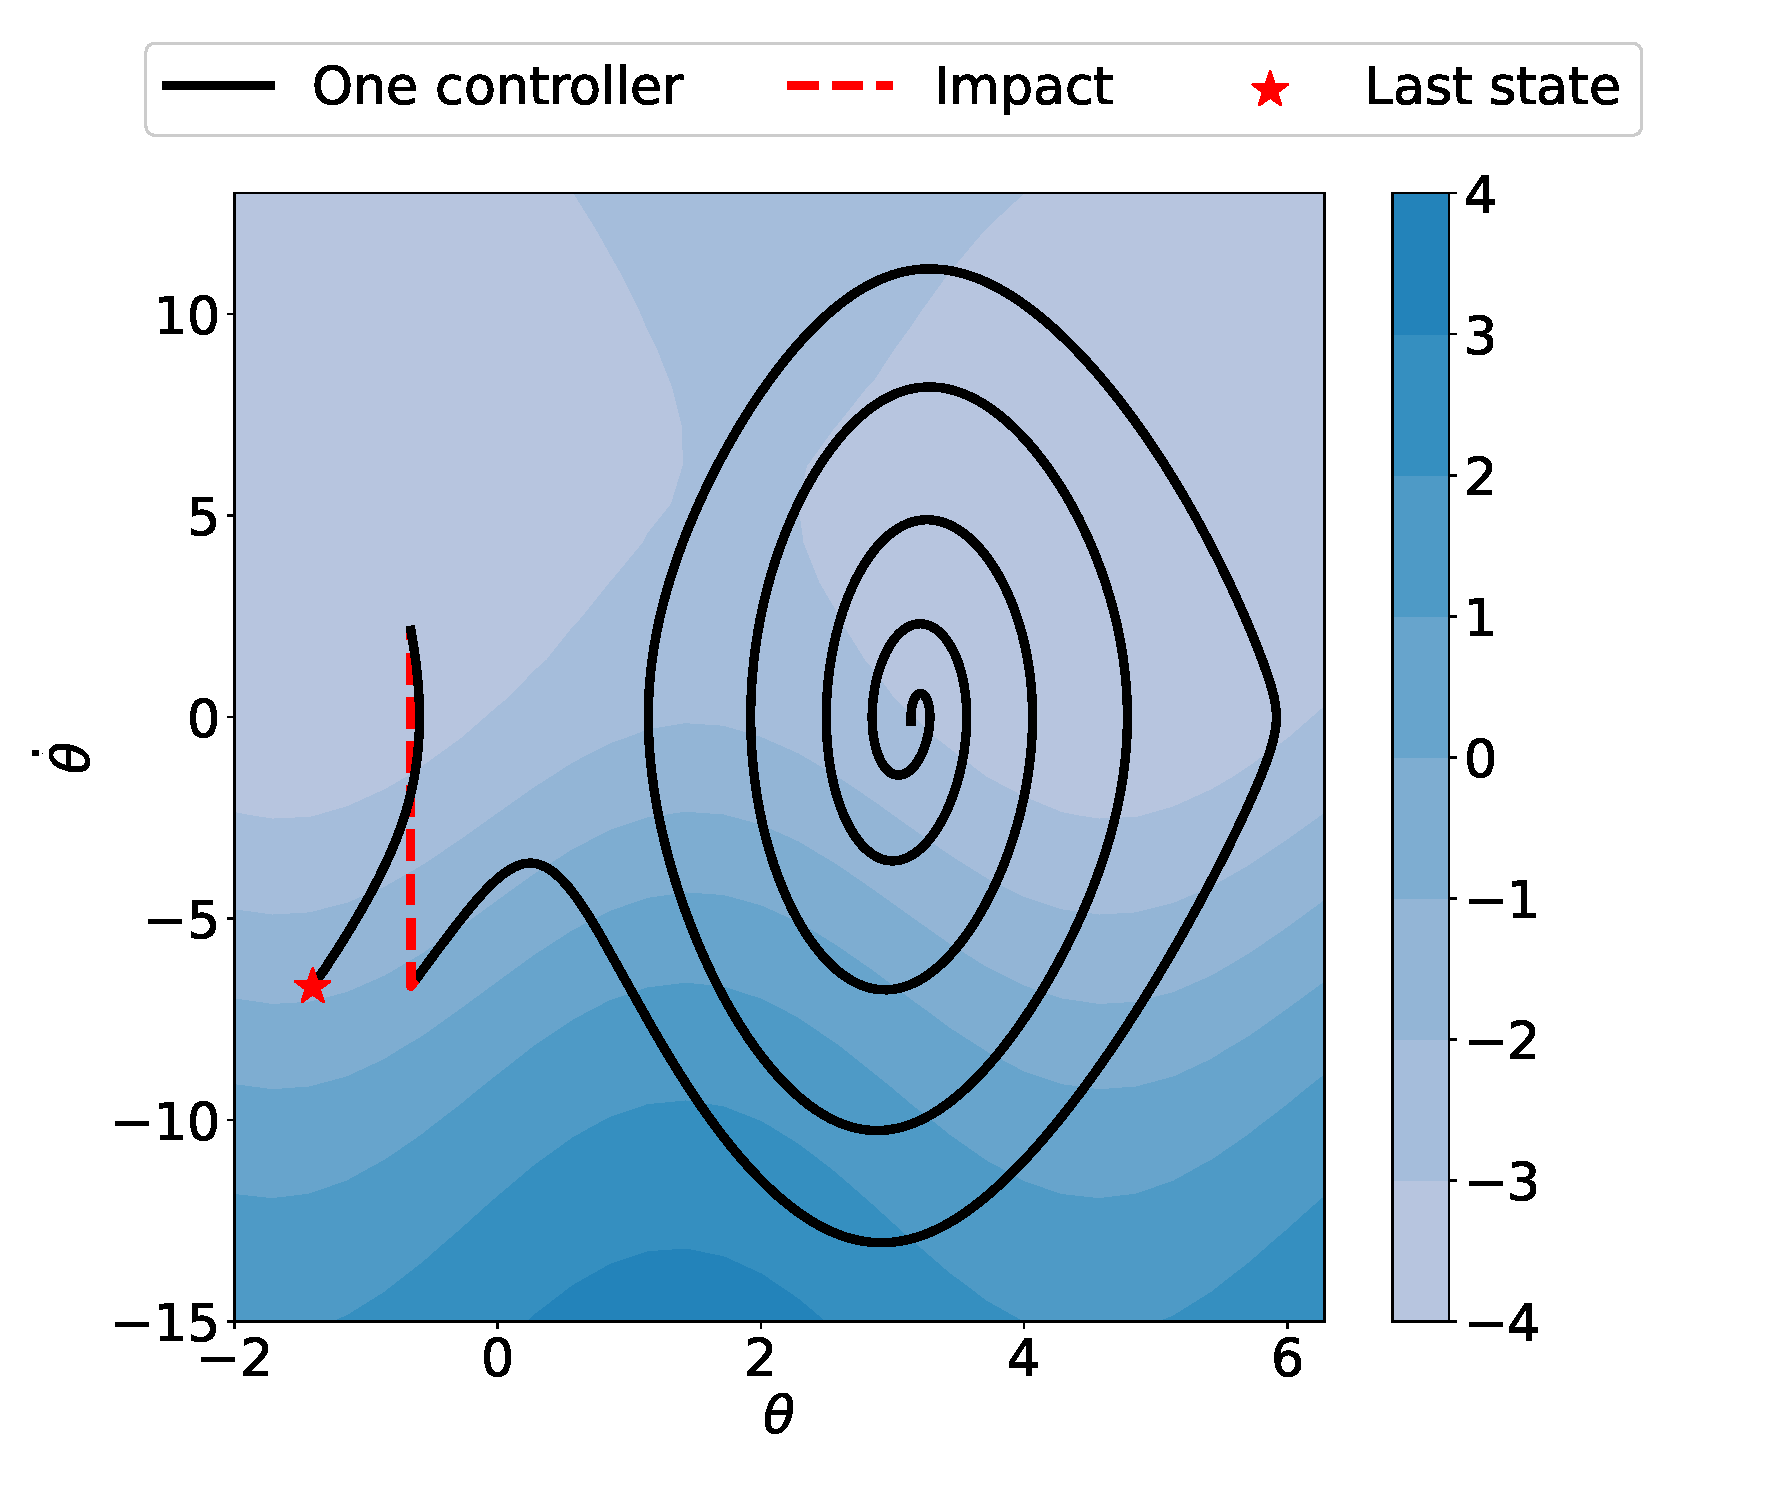
\includegraphics[width=0.7\linewidth]{cont.eps}
    \caption{A sample trajectory generated by the single controller. }
    \label{fig:continuous_control}
\end{figure}

\begin{figure}[H]
    \centering
    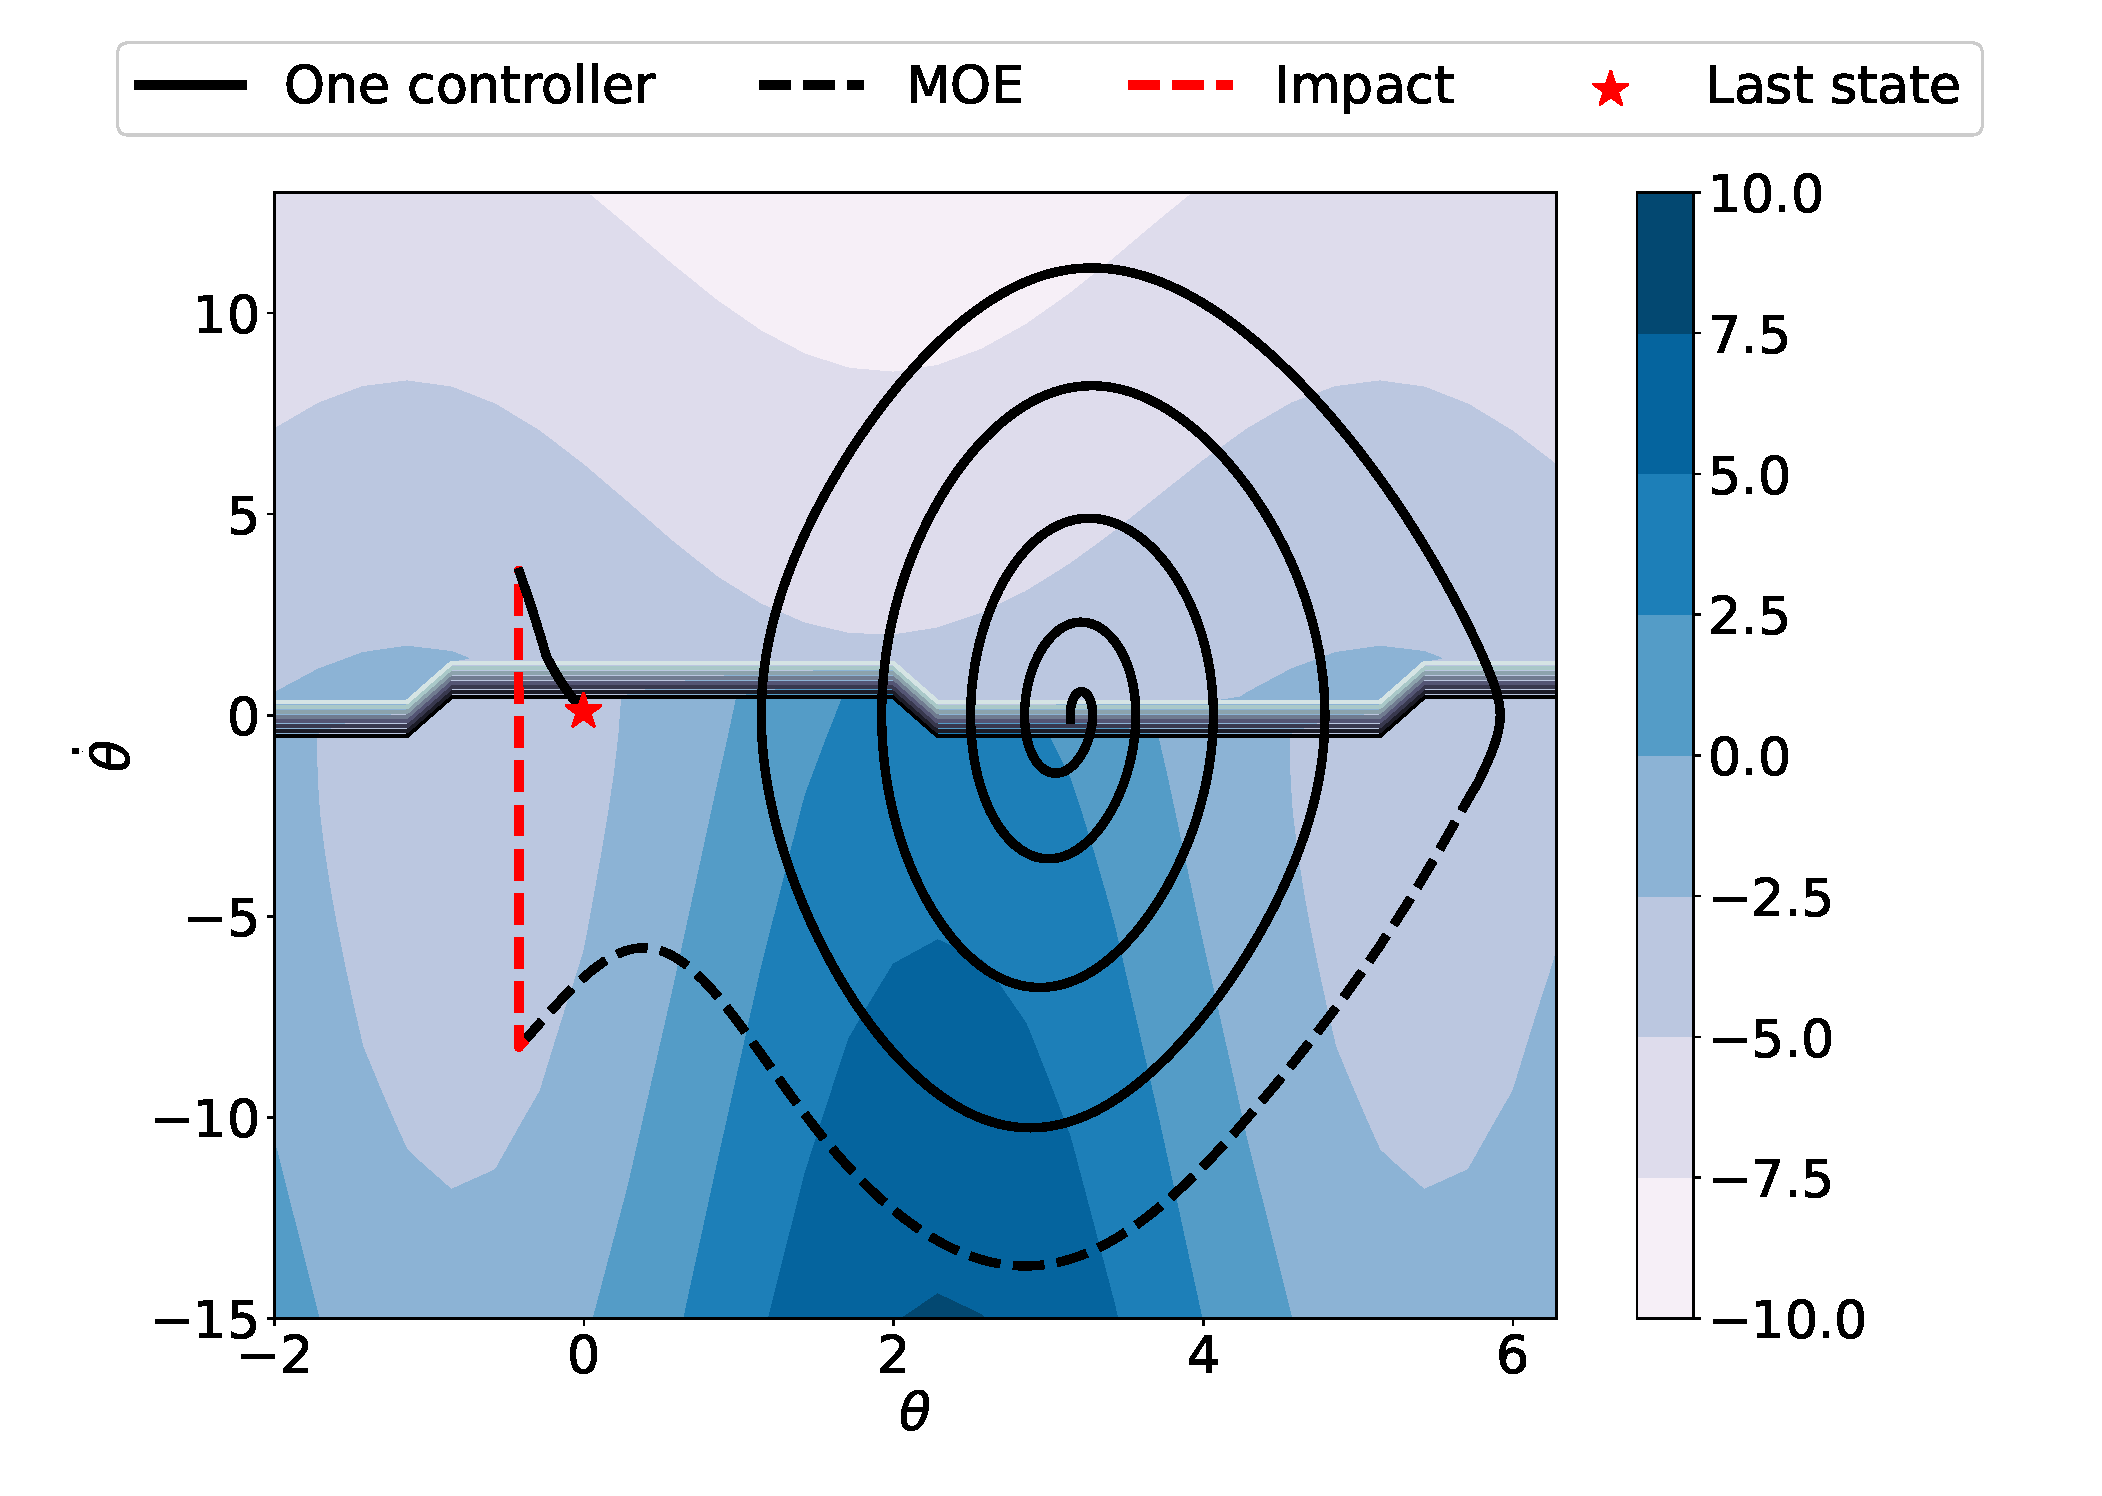
\includegraphics[width=0.7\linewidth]{contANDMOE.eps}
    \caption{The performance of the MOE controllers compared to the single
    controller in Figure~\ref{fig:continuous_control}}.
    \label{fig:contandmoe}
\end{figure}
